\clearpage

\section{Frequency Mismatch Compensation}
\label{sec:frequency_mismatch_compensation}
\begin{refsection}

\begin{tcolorbox}	
\begin{tabular}{p{2.75cm} p{0.2cm} p{10.5cm}} 	
\textbf{Header File}    &:& frequency\_mismatch\_compensation\_*.h \\
\textbf{Source File}    &:& frequency\_mismatch\_compensation\_*.cpp \\
\textbf{Version}        &:& 20190114 (Daniel Pereira)
\end{tabular}
\end{tcolorbox}

\subsection*{Input Parameters}

\begin{table}[H]
\centering
\begin{tabular}{|l|l|l|}
\hline
Name                         & Type           & Default Value \\ \hline
pilotRate                    & integer        & 0             \\ \hline
numberOfSamplesForEstimation & integer        & 21            \\ \hline
\end{tabular}
\end{table}


\subsection*{Methods}

\begin{itemize}
  \item FrequencyMismatchCompensation(vector<Signal *> \&InputSig, vector<Signal *> \&OutputSig) :Block(InputSig,OutputSig)\{\};
  \item void initialize(void);
  \item bool runBlock(void);
  \item void setPilotRate(int pRate) \{ pilotRate = pRate; \};
  \item void setNumberOfSamplesForEstimation(int nSamplesEstimation) \{ numberOfSamplesForEstimation = nSamplesEstimation; samplesForEstimation.resize(nSamplesEstimation); \};
  \item void setMode(FrequencyCompensationMode m) \{  mode = m; \}
\end{itemize}




\subsection*{Input Signals}

\textbf{Number}: 1\\
\textbf{Type}: Complex (DiscreteTimeContinuousAmplitude)


\subsection*{Output Signals}

\textbf{Number}: 1\\
\textbf{Type}: Complex (DiscreteTimeContinuousAmplitude)

\subsection*{Functional Description}

This block accepts a complex constellation and outputs another built from its input. The block attempts to perform frequency mismatch compensation on the input constellation by one of three different methods:
\begin{itemize}
\item Pilot aided method
\item Blind estimation method
\item Spectral method
\end{itemize}

\subsection*{Theoretical Description}



The signal at the receiver for a system with frequency mismatch can be assumed to take the form
\begin{equation}\label{eq:signalWithFrequencyMismatch} 
y(t)=|y(t)|e^{i[\Delta\omega t+\theta(t)+\epsilon(t)]}, 
\end{equation}
where $\Delta\omega$ is the frequency mismatch, $\theta(t_n)$ is the phase encoded in the signal and $\epsilon(t_n)$ is the phase noise contribution.
Frequency mismatch compensation	is accomplished by first estimating the value of $\Delta\omega$ and then removing via
\begin{equation}
y(t)^\prime=y(t)*e^{-i\Delta\hat{\omega}}.
\end{equation}
\par
Three methods for estimating $\Delta\omega$ are presented here.

\subsubsection*{Pilot aided frequency mismatch compensation}

This method uses a pilot signal similar to the ones employed in pilot assisted phase mismatch compensation techniques. In an pilot aided technique a reference signal (the pilot), composed of pre-agreed on symbols, is inserted, time multiplexed, with the data payload at a pre-agreed on rate. A visual representation of the output of the modulation stage of a pilot-assisted scheme is presented in Figure~\ref{fig:pilotMethodExplanation}.
\begin{figure}[h]
\centering
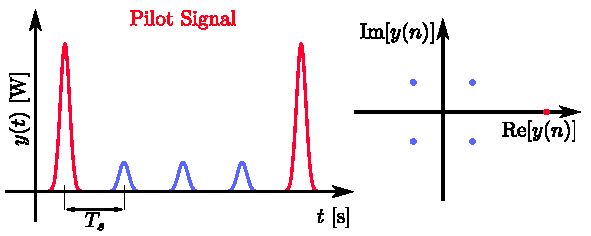
\includegraphics{./lib/frequency_mismatch_compensation/figures/novelMethodConstellation.pdf}
\caption{Time dependence (left) and constellation (right) at the output of the modulation stage of a pilot-assisted scheme. Pilot pulses/points identified by color. Pilot rate in the time dependence image is meant only as illustrative, actual pilot rate may be higher or lower.}
\label{fig:pilotMethodExplanation}
\end{figure}
At the receiver stage, after coherent detection, the signal is described by
\begin{equation}\label{eq:signalAfterCoherentDetection} 
y(t_n)=
\begin{cases}
x_s(t_n)e^{i[\Delta\omega t_n+\theta_q(t_n)+\epsilon(t_n)]},~n\neq mR_P \\
x_p(t_n)e^{i[\Delta\omega t_n+\epsilon(t_n)]},~n=mR_P
\end{cases},
\end{equation}
where $x_s(t)$/$x_p(t)$ represents the signal/pilot amplitude, $R_P$ is the pilot rate, $\Delta\omega$ is the offset frequency, $\epsilon(t)$ is the instantaneous phase noise contribution and $\theta(t)$ is the phase modulation at instant $t$. The first step in this technique is to obtain the auxiliary signal $x_f(m)$, which is defined as
\begin{equation}\label{eq:xfreq}
\begin{aligned}
x_f(m)&=y_r^*(t_{mR_P})y_r(t_{(m+1)R_P})\\
&=x_p(t_{mR_p})x_p(t_{(m+1)R_p})e^{i\left(\Delta\omega R_PT_s+\Delta\epsilon(m)\right)},
\end{aligned}
\end{equation}
where
\begin{equation}
\Delta\epsilon(m)=\epsilon(t_{mR_P})-\epsilon(t_{(m+1)R_P}).
\end{equation}
The frequency estimation is accomplished by taking the expected value of the complex argument of~\eqref{eq:xfreq} and dividing it by $R_PT_s$. This returns
\begin{equation}\label{eq:omegaEst}
\begin{aligned}
\Delta\hat{\omega}&=\operatorname{E}\left[\frac{1}{R_PT_s}\text{arg}(x_f(m))\right]\\
&=\operatorname{E}\left[\Delta\omega+2k\pi(R_PT_s)^{-1}+\frac{\Delta\epsilon(m)}{R_PT_s}\right]\\
&=\Delta\omega+2k\pi(R_PT_s)^{-1}.
\end{aligned}
\end{equation}

\subsubsection*{Blind estimation frequency mismatch compensation}

In this method the frequency is scanned over a predetermined range, symbol decisions are made and the minimum square error used as the frequency-selection criteria. Scanning is first done with a large step to find a rough value for $\Delta\omega$, this is then repeated with a smaller step to find a more exact estimate~\cite{zhou11}.

\subsubsection*{Spectral evaluation frequency mismatch compensation}

In this method the frequency is estimated by evaluating the spectrum of the mth power of the input signal~\cite{selmi09}, which exhibits a peak at the frequency $m\Delta\Omega$, this value is used as the estimate.


% bibliographic references for the section ----------------------------
\clearpage
\printbibliography[heading=subbibliography]
\end{refsection}
\addcontentsline{toc}{subsection}{Bibliography}
\cleardoublepage
% --------------------------------------------------------------------- 